\section{Method}
In this section, we outline the scaling strategies from three perspectives. In Section \ref{sec:model_scaling}, we detail the scaling strategies of the folding models. In Section \ref{sec:linear_att}, we propose a novel triangular attention module as a drop-in replacement for the vanilla triangular attention module. In Section \ref{sec:data_scaling}, we present the dataset crawled for training \texttt{SeedFold}.

\begin{figure}[t]
    \centering
    \begin{subfigure}{\linewidth}
        \centering
        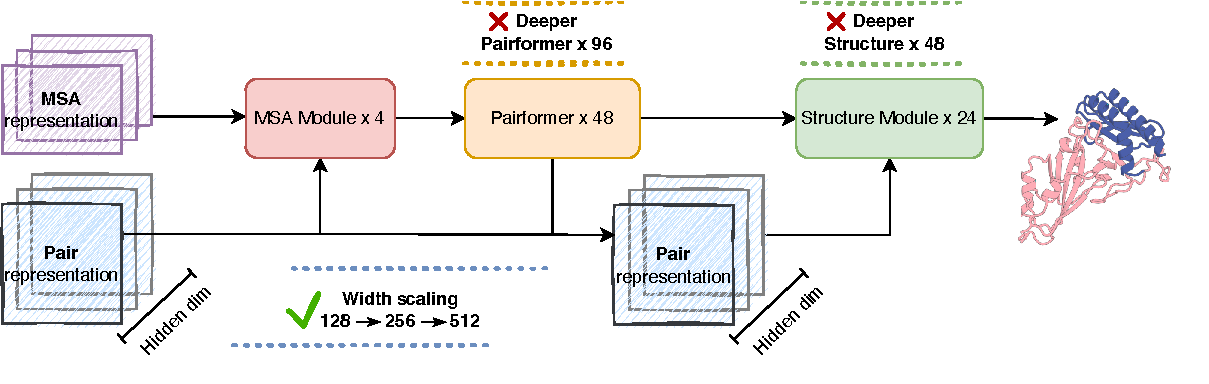
\includegraphics[width=0.85\linewidth]{figures/model_arch_horizon_v2.pdf}
        \caption{Model architecture and scaling strategies.}
        \label{fig:arch}
    \end{subfigure}
    \vspace{1em}
    \begin{subfigure}{\linewidth}
    \centering
        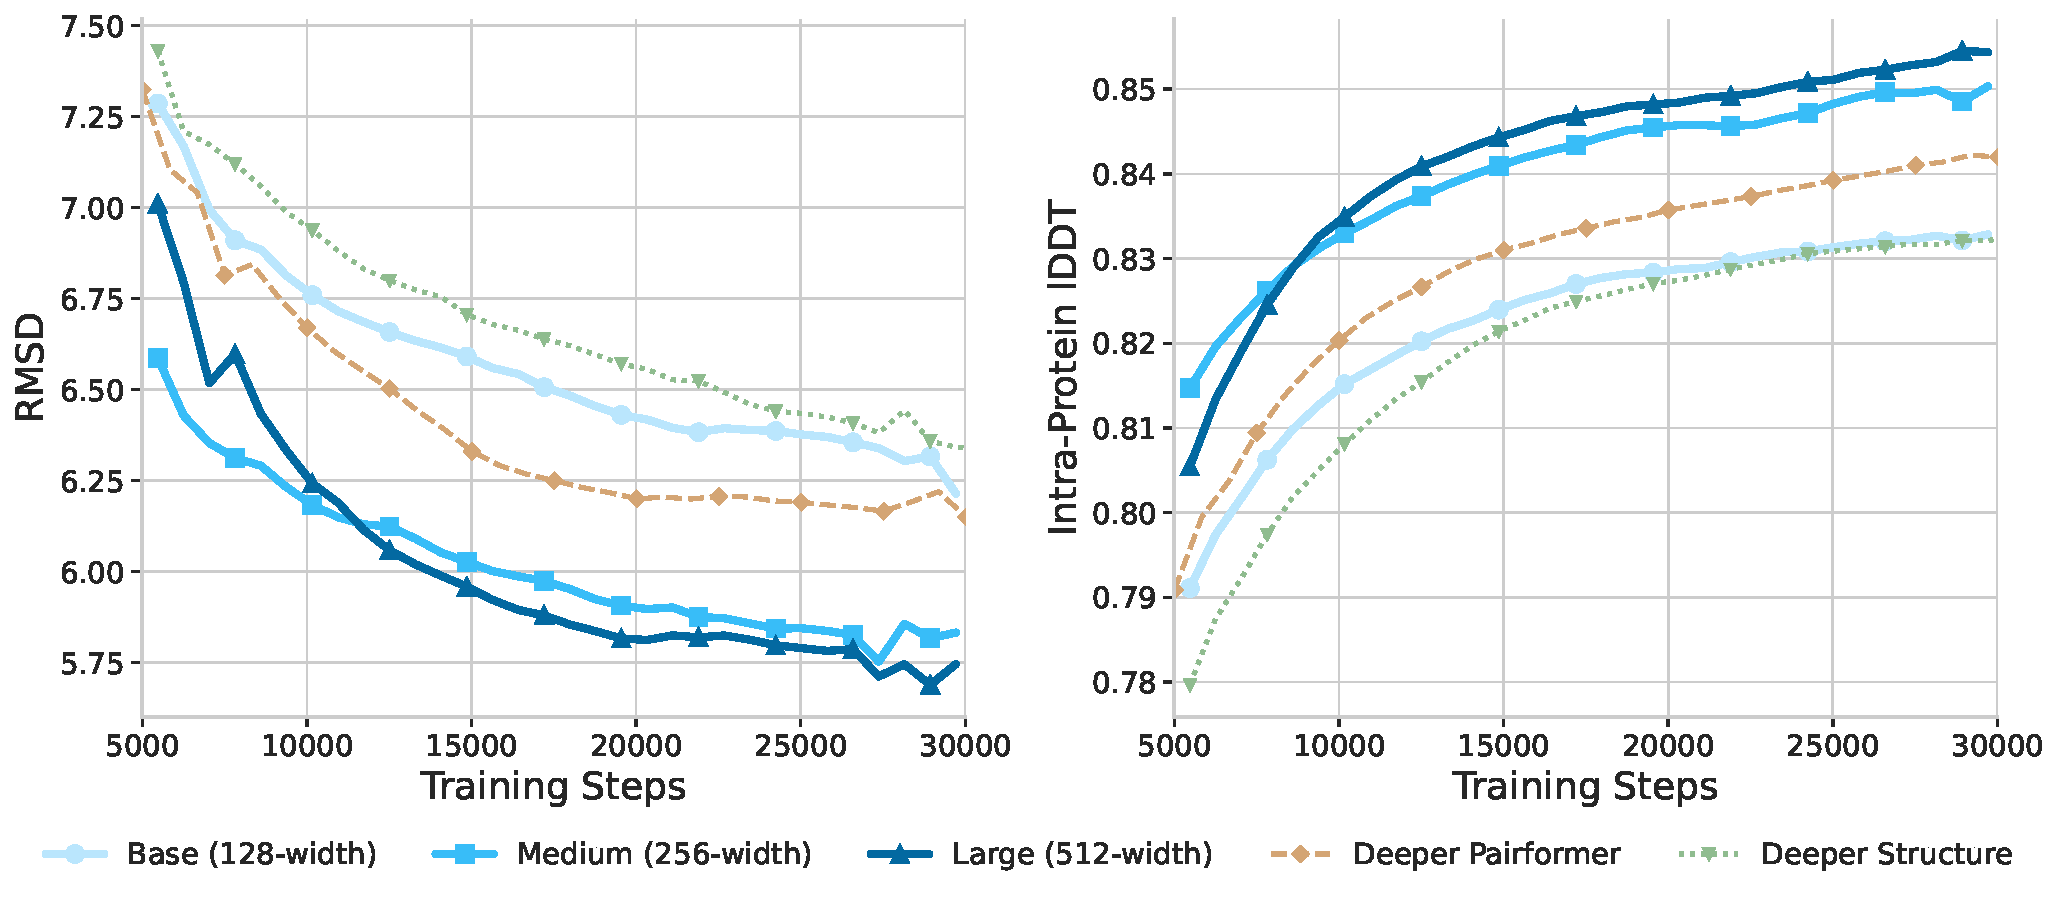
\includegraphics[width=0.8\linewidth]{figures/scale_up_combined.pdf}
        \caption{Comparsion of different scaling strategies.}
        \label{fig:scaling_data}
    \end{subfigure}
    \caption{Comparison of different scaling strategies. (a) Conceptual illustration of the scaling strategy.(b) Performance comparison where the left plot shows complex RMSD (lower is better) for global structural accuracy, and the right plot shows intra-protein lDDT (higher is better) for local structural quality. Width scaling consistently outperforms depth scaling. The transition from Small ($128$-width) to Medium ($256$-width) yields the largest gains in both global RMSD and local lDDT, while further scaling to Large ($512$-width) shows diminishing returns. Deeper trunk and deeper structure module provide marginal improvements compared to width scaling.}
    \label{fig:scaling_combined}
\end{figure}




\subsection{Model Scaling}
\label{sec:model_scaling}

The capacity of current folding models is primarily bottlenecked by the hidden dimension of the pair representation. While previous works have mainly focused on scaling the number of Pairformer layers~\cite{passaro2025boltz,bytedance2025protenix}, this work investigates scaling the hidden dimension, hypothesizing it to be more effective for representation learning. To explore the upper bound of model capacity, the model is systematically scaled up by increasing the pair representation dimension from $128$ to $512$, with a corresponding expansion in the MSA module to provide richer evolutionary features.

\paragraph{Model Architecture Overview}
Several strategies can be explored for model scaling. The folding model primarily consists of two modules: the trunk module and the structure module. The trunk module is mainly composed of the MSA module and the Pairformer module. The MSA module samples diverse MSAs through different recycles and extracts evolutionary features, which are then used to update the pair representation; conversely, the learned pair representation is also used to update the MSA hidden representation. The Pairformer module updates pair representations through pairwise triangular multiplication and triangular attention to capture inter-token interactions. The structure module takes the pair and single representations encoded by the trunk module as conditions to perform all-atom structure generation.

\begin{table}[t]
    \centering
    \caption{Model configurations at different scales. We explore scaling strategies for folding models by varying the trunk width (pair and MSA dimensions), trunk depth (Pairformer layers), and structure module depth. Training efficiency is measured on the same GPU type for fair comparison.}
    \label{tab:model_scaling}
    % \resizebox{\linewidth}{!}{
    \begin{tabular}{lcccccc}
        \toprule
        % \textbf{Configuration} & \textbf{Pair Dim} & \textbf{MSA Dim} & \textbf{\#Pairformer Layers} & \textbf{\#Structure Layers} & \textbf{\#Params} & \textbf{Efficiency (iters/s)} \\
        \textbf{Configuration} & \textbf{\makecell{Pair Rep.\\Dim}} & \textbf{\makecell{MSA Rep.\\Dim}} & \textbf{\makecell{Pairformer\\Layers}} & \textbf{\makecell{Structure\\Layers}} & \textbf{\makecell{\#Params}} & \textbf{\makecell{Efficiency\\(iters/s)}} \\

        \midrule
        Base (128-width) & $128$ & $64$ & $48$ & $24$ & $432$M & $0.15$ \\
        Medium (256-width) & $256$ & $128$ & $48$ & $24$ & $533$M & $0.10$ \\
        Large (512-width) & $512$ & $256$ & $48$ & $24$ & $923$M & $0.06$ \\
        \midrule
        Deep Pairformer & $128$ & $64$ & $96$ & $24$ & $582$M & $0.10$ \\
        Deep Structure Module & $128$ & $64$ & $48$ & $48$ & $706$M & $0.10$ \\
        \bottomrule
    \end{tabular}
    % }
\end{table}

% \paragraph{Design Space}
% Based on this architecture, we can explore scaling along several dimensions:
% \begin{itemize}
%     \item \textbf{Width vs. Depth}: We can choose between deeper or wider networks. In terms of depth, we can increase model capacity by adding more Pairformer layers. Alternatively, we can scale up by increasing the dimension of the pair representation.
%     \item \textbf{Trunk vs. Structure Module}: The folding model can be conceptualized as an encoder-decoder architecture, in which the Pairformer functions as the encoder and the score module acts as the decoder. We argue that the encoder requires more capacity~\cite{kasai2020deep}, i.e., the Pairformer, since it serves a representation learning role, where the learned pair and single representations drive the structure module to decode all-atom structures.  Therefore, we can either expand the trunk module to enhance representation capability, or enlarge the structure module to improve structure generation capacity. 
%     % \todoq{do you imply pairformer is trunk module? btw, trunk module is not defined up to this place} 
% \end{itemize}

\paragraph{Scaling Strategy}
We construct three types of models to investigate different scaling strategies. Table~\ref{tab:model_scaling} presents the basic configurations of our scaling experiments. Figure~\ref{fig:scaling_combined} shows the results of different scaling strategies.

\begin{itemize}
    \item \textbf{Wider Trunk}: We scale the trunk width, i.e., the MSA module and the Pairformer width, as they work together to build rich pair representations. Specifically, we progressively increase the MSA hidden dimension from $64$ to $256$, while simultaneously increasing the dimension of pair representation from $128$ to $512$. The Pairformer parameter count scales from $147$M to $549$M, and the overall model size grows from $430$M to approximately $1$B. The corresponding training efficiency is shown in Table~\ref{tab:model_scaling}. 
    When scaling from Base ($128$-width) to Medium ($256$-width), we observe significant improvements across all metrics, including overall lDDT and RMSD that reflects global structural accuracy. When further scaling from Medium to Large ($512$-width), we adjust the optimization hyperparameters to stabilize training. The model still demonstrates consistent improvements on the test set, although the gains are less pronounced compared to the Base-to-Medium transition, suggesting diminishing returns at larger scales.
    
    \item \textbf{Deeper Trunk}: We increased the number of Pairformer layers from $48$ to $96$. This approach yielded a less significant performance gain compared to width scaling. This result is not surprising, as the use of $9$ recycling iterations with a $48$-layer network already creates a very deep effective architecture. Further increasing the physical depth is thus expected to offer diminishing returns. This observation is analogous to findings in large language models, where techniques like early exiting can skip later layers to accelerate inference with minimal impact on performance~\cite{elhoushi2024layerskip}.
    % \todoq{deep is confusing. it implies 48 is not deep, 96 is deep?}
    
    \item \textbf{Deeper Structure Module}: We increase the token transformer layers in the structure module from $24$ to $48$. This yields the lowest observed improvement among all scaling strategies. This is as expected, as the structure is largely determined by the pair representation, while the structure module functions more as a ``translator'' to convert a pair representation into coordinates~\cite{lin2023evolutionary}, which is a relatively easier task.
    % \todoq{deep is confusing. it implies 24 is not deep, 48 is deep?}
\end{itemize}

These results suggest that width scaling of the Pairformer is the most effective strategy for improving folding model performance. The pair representation dimension appears to be the critical bottleneck: increasing it directly enhances the model's capacity to encode complex pairwise interactions. In contrast, depth scaling of either the trunk or structure module provides diminishing returns, indicating that the representation capacity, rather than the number of processing steps, is the primary limiting factor.















\subsection{Linear Triangular Attention}
\label{sec:linear_att}

A scalable foundational component is essential for scaling folding models. At present, the main computational bottleneck of folding models occurs in the triangular operations, in particular within \texttt{TriangularAttention}. The module updates the pair representation $\mathbf{Z} \in \mathbb{R}^{n\times n \times d}$ in a manner similar to ``row-wise/column-wise attention with bias''. Denote the $i$-th row of $\mathbf{Z}$ as $\mathbf{Z}_i \in \mathbb{R}^{n\times d}$, the triangular attention on the $i$-th row can be computed by:
\begin{align}
\mathbf{Q}_i, \mathbf{K}_i, \mathbf{V}_i & = \mathtt{Linear}(\mathbf{Z}_i) \in \mathbb{R}^{n\times d} \\
\mathbf{B} & = \mathtt{Linear}(\mathbf{Z}) \in \mathbb{R}^{n\times n} \\
\mathtt{TriAtt}(\mathbf{Z}_i) & = \mathtt{softmax}\left(\mathbf{Q}_i\mathbf{K}_i^T+\mathbf{B}\right)\mathbf{V}_i,
\end{align}
where we omit the $\sqrt{d}$ in the attention for simplicity. Computing the attention scores for each row and column requires materializing a large matrix $(\mathbf{Q}_i\mathbf{K}_i^T+\mathbf{B}) \in \mathbf{R}^{n\times n}$, a cost that becomes particularly evident when the dimension of the row is taken into account and the complexity increases to  $\mathcal{O}(n^3d)$. 



\begin{figure}[t]
    \centering
    \begin{subfigure}[t]{0.4\linewidth}
        \centering
        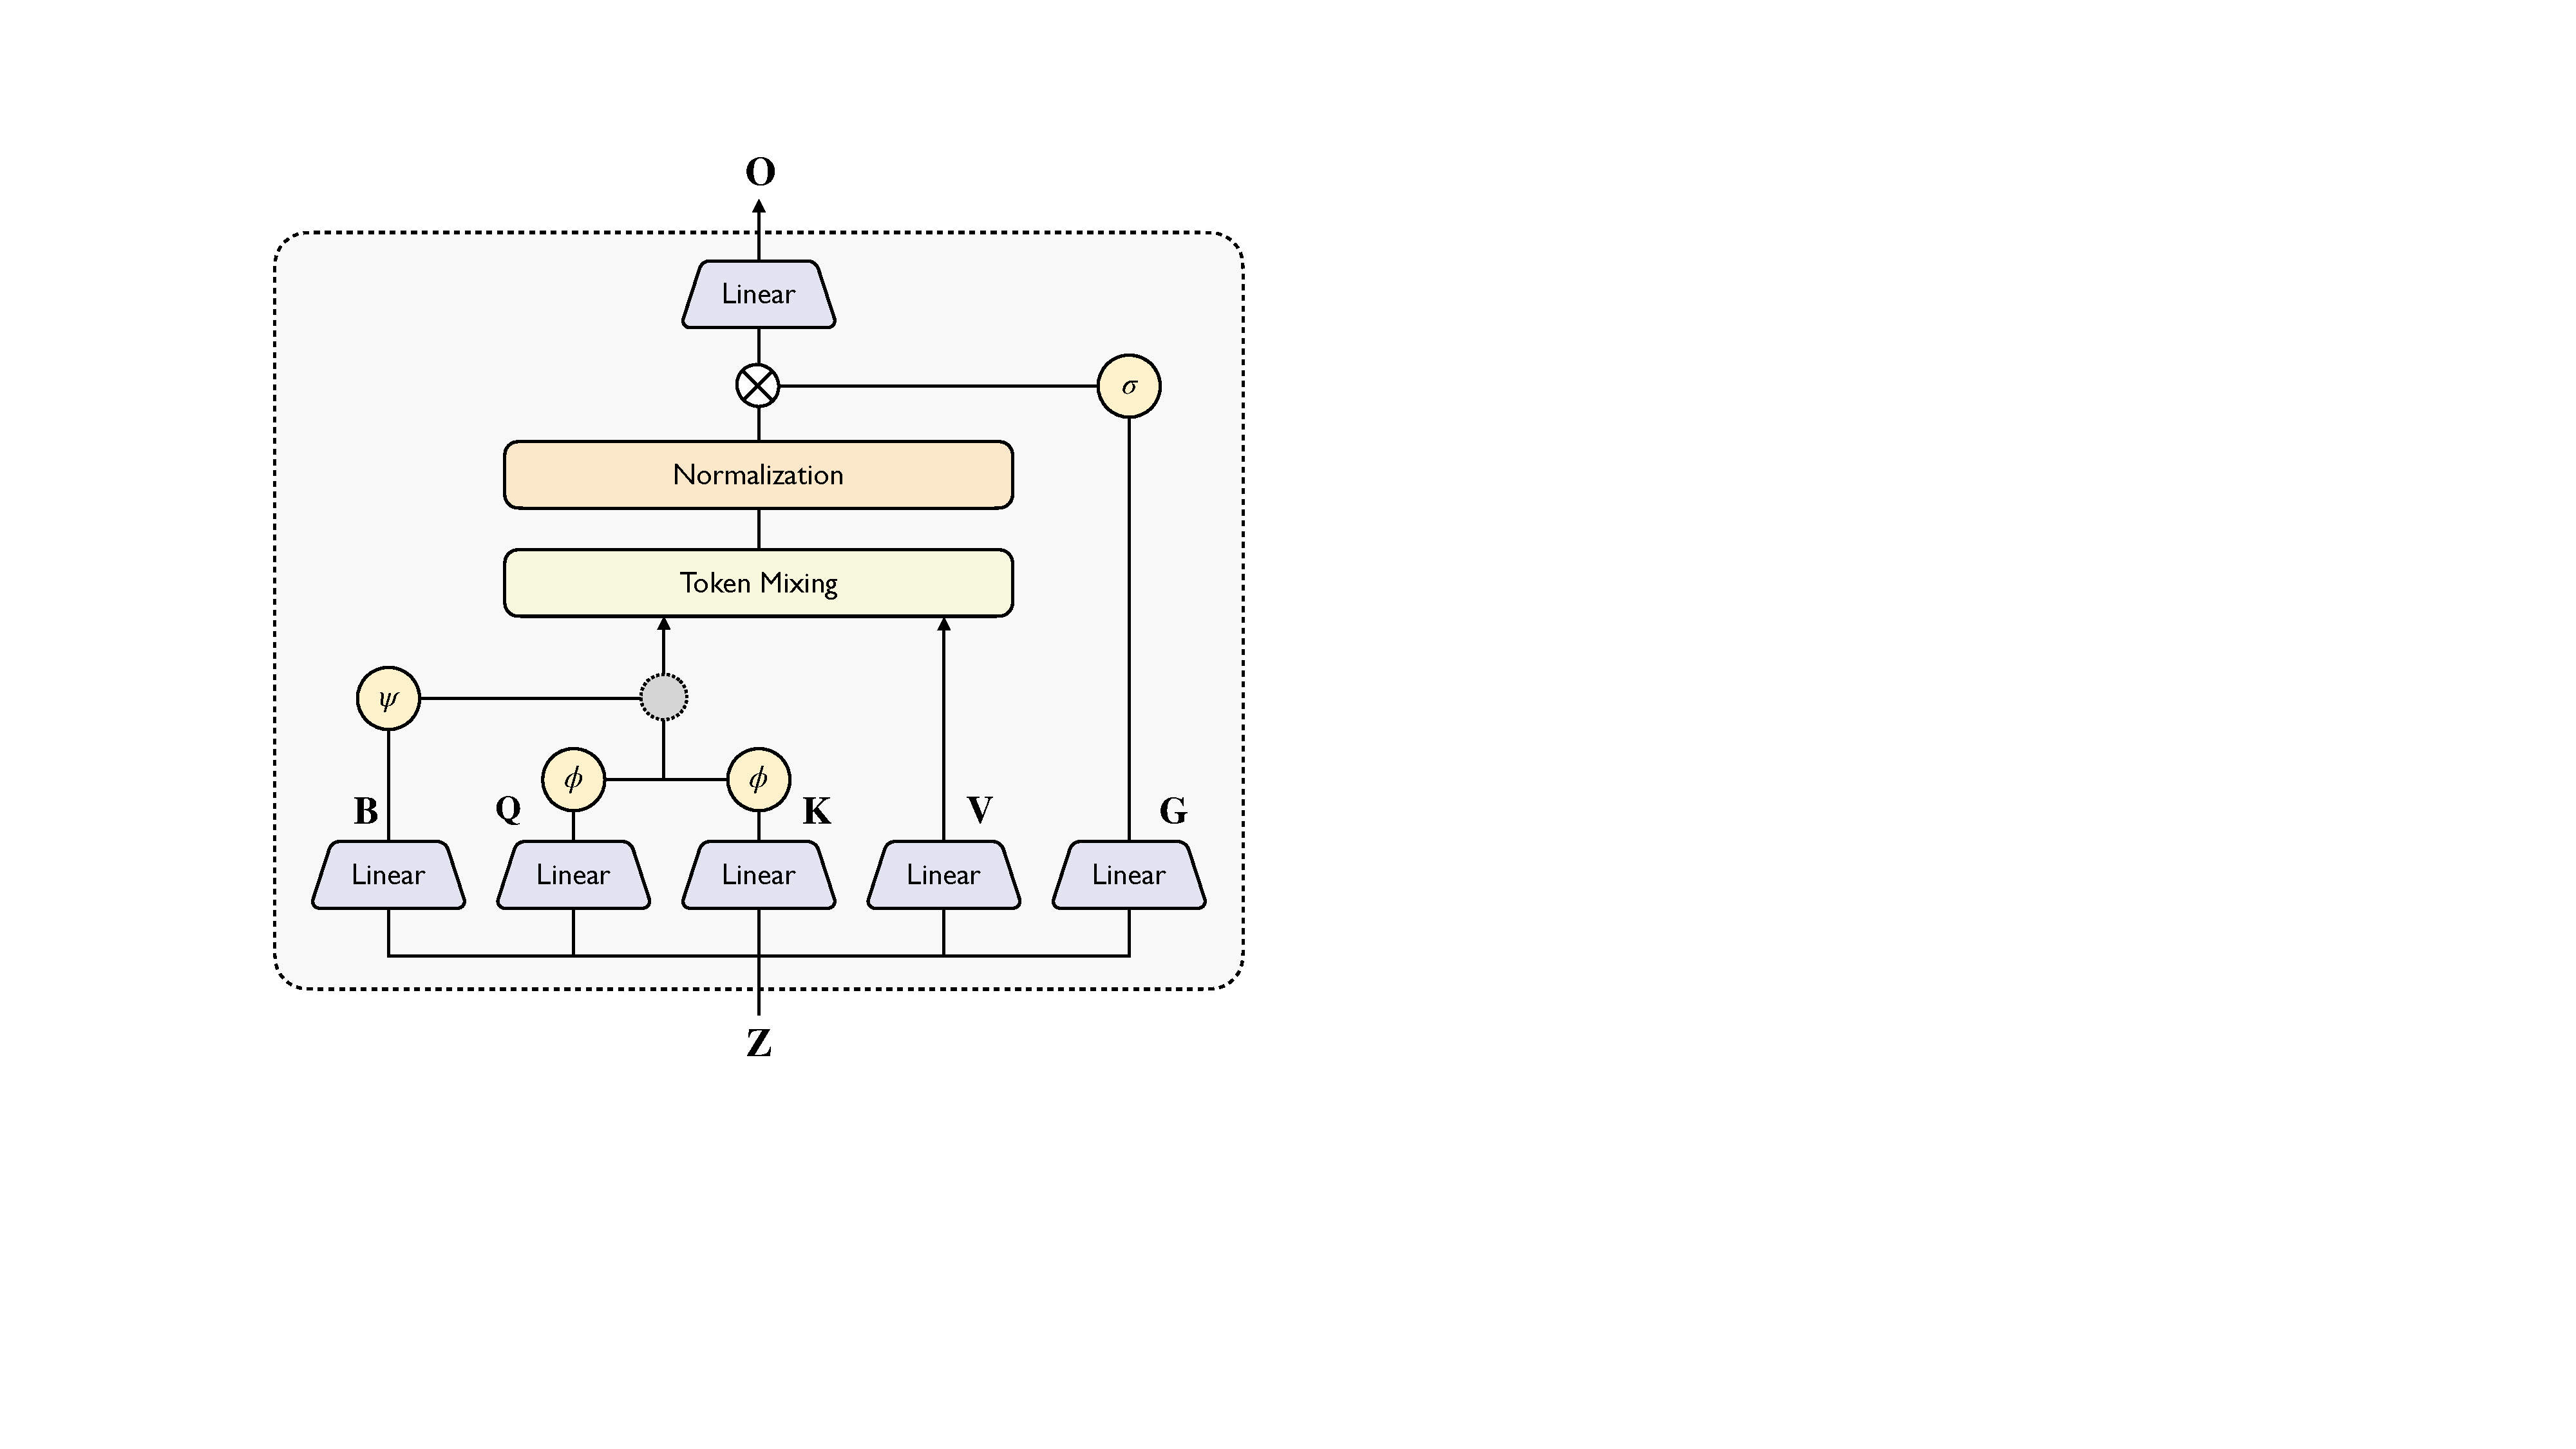
\includegraphics[width=\linewidth]{figures/linear_attention.pdf}
        \caption{}
        % \caption{The architecture of the linear attention module.}
        \label{fig:linear_attention}
    \end{subfigure}
    \hfill
    \begin{subfigure}[t]{0.55\linewidth}
        \centering
        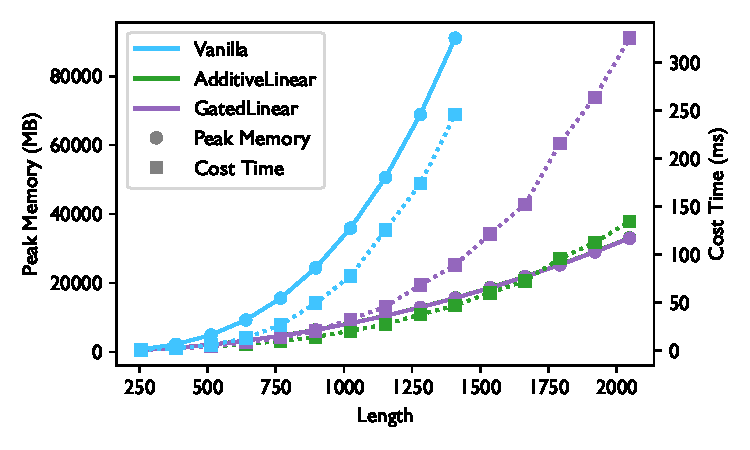
\includegraphics[width=\linewidth]{figures/bench_kernel.pdf}
        \caption{}
        % \caption{The peak memory usage (MB) and time cost (ms) of different attention modules. The two linear attention mechanisms have similar peak memory usages, which overlap in the figure.}
        \label{fig:bench_kernel}
    \end{subfigure}
    \caption{The \texttt{LinearTriangularAttention} module. (a) The architecture of the linear attention module. (b) The peak memory usage (MB) and time cost (ms) of different attention modules. Two linear attention mechanisms have similar peak memory usages, which overlap in the figure.}
    % \label{fig:attention_summary}
\end{figure}



We aim to reduce complexity by introducing linear attention, which is a modern memory-saving technique widely adopted in large language models~\cite{minimax2025minimax01scalingfoundationmodels,kimiteam2025kimilinearexpressiveefficient}. The theoretical background of linear attention lies in the use of well-established random feature maps $\phi(\cdot)$ to approximate the ``dot-then-exponentiate'' function via the inner product $\mathtt{exp}(\mathbf{x}, \mathbf{y})\approx\langle\phi(\mathbf{x}), \phi(\mathbf{y})\rangle$ ~\cite{rahimi2007random,peng2021randomfeatureattention}. In practice, this is further simplified by directly substituting the \texttt{softmax} kernel with a simple non-linear feature map (e.g., $\mathtt{relu(\cdot)}$, $1+\mathtt{elu(\cdot)}$, $\mathtt{silu}(\cdot)$), where the attention operation $\mathtt{softmax}(\mathbf{Q}_i\mathbf{K}_i^T)\mathbf{V}_i$ is replaced by $\phi(\mathbf{Q}_i)\phi(\mathbf{K}_i)^T\mathbf{V}_i$. Such a reformulation offers a significant benefit, as it enables the application of the right product trick to reduce computational complexity. By first computing the right matrix multiplication, the computational cost can be reduced from $\mathcal{O}(n^2d)$ to  $\mathcal{O}(nd^2)$:
\begin{align}
\underbrace{\phi(\mathbf{Q}_i)\phi(\mathbf{K}_i)^T}_{\mathcal{O}(n^2d)}\mathbf{V}_i
\rightarrow \phi(\mathbf{Q}_i)\underbrace{\phi(\mathbf{K}_i)^T\mathbf{V}_i}_{\mathcal{O}(nd^2)}.
\end{align}
However, the original formulation of linear attention does not incorporate the bias term, which is essential for folding models to perform geometric reasoning in 3D space. Since $\mathbf{Z}_{ij}$ stores the coupling between the $i$-th and $j$-th tokens, $\mathbf{Q}_{ij}\mathbf{K}_{ik}$ quantifies the correlation between the $(i,j)$-th coupling and the $(i,k)$-th coupling. AlphaFold enhances the attention mechanism through the introduction of an additive bias, yielding a triangular form that also accounts for the $(j,k)$-th coupling: $\mathbf{Q}_{ij}\mathbf{K}_{ik}+\mathbf{B}_{jk}$.
We propose to convert the linear attention into a triangular form where the attention scores can be reweighted.
\begin{align}
    \mathtt{LinearTriAtt}(\mathbf{Z}_i) = \left(\phi(\mathbf{Q}_i)\phi(\mathbf{K}_i^T)\Box\psi(\mathbf{B})\right)\mathbf{V}_i,
\end{align}
where $\phi$ and $\psi$ are two feature maps and $\Box$ denotes an undefined operation. We present two choices for the boxed operation $\Box$: (i) an additive operation $+$ that up-weights or down-weights the attention score, similar to AlphaFold. (ii) a multiplication operation $\times$ that functions as a gating mechanism to control the information flow.

\paragraph{Additive Linear Triangular Attention} The additive operation inherits all the advantages of the vanilla version, which holds the potential to facilitate the adoption of well-established designs from modern linear attention. 
\begin{align}
    \mathtt{AdditiveLinearTriAtt}(\mathbf{Z}_i) & = \left(\phi(\mathbf{Q}_i)\phi(\mathbf{K}_i^T)+\psi(\mathbf{B})\right)\mathbf{V}_i \\
    & = \phi(\mathbf{Q}_i)\underbrace{\left(\phi(\mathbf{K}_i^T)\mathbf{V}_i\right)}_{\text{linearized}} +\underbrace{\psi(\mathbf{B})\mathbf{V}_i}_{\text{amortized}}.
\end{align}
It is worth noting that although we highlight the advantage of linear attention in avoiding the materialization of the $\mathbb{R}^{n\times n}$ attention matrix, the bias term in this variant is still structured as $\mathbb{R}^{n\times n}$. However, since triangular attention is performed for each row, its complexity is actually $\mathcal{O}(n\times n^2)$, where the first $n$ is the number of rows. With regard to the bias term, it is shared across all rows; that is, the memory usage can be amortized and does not grow with $n$. In our implementation, we choose $\phi=\mathtt{relu}$ and $\psi=\mathtt{relu}$.

\paragraph{Gated Linear Triangular Attention} The gated variant is more intuitive for controlling the information flow, i.e., we adopt a gating function $\psi:\mathbf{B}_{jk}\mapsto[0,1]$ to decide how much correlation exists between $\mathbf{Q}_{ij}$ and $\mathbf{K}_{ik}$.
\begin{align}
    \mathtt{GatedLinearTriAtt}(\mathbf{Z}_i) = \left(\phi(\mathbf{Q}_i)\phi(\mathbf{K}_i^T)\odot\psi(\mathbf{B})\right)\mathbf{V}_i, 
\end{align}
where $\odot$ denotes the pointwise matrix multiplication, which serves a role analogous to that of the (causal) attention mask in large language models. Unfortunately, the $\odot$ operation disrupts the matrix chain product, which means we cannot adopt the right product trick. To mitigate this issue, we develop a tiled version of linear attention which is optimized for reducing the memory footprint on CUDA devices~\cite{dao2022flashattentionfastmemoryefficientexact,Atkinson2025latkins,Geiger2025NVIDIA}. We refer the readers to Appendix~\ref{appendix:triton} for detailed information. In our implementation, we choose $\phi=\mathtt{relu}$ and $\psi=\mathtt{sigmoid}$.


Putting everything together, we developed two variants of linear triangular attention to mix information between tokens. The architecture of this module is illustrated in Figure~\ref{fig:linear_attention}. We further perform normalization and gating on the output following Lightning Attention, which has proven its effectiveness in industry-level large language models~\cite{qin2024lightning, qin2024transnormerllm, minimax2025minimax01scalingfoundationmodels}, i.e., $\mathtt{Linear}(\sigma(\mathtt{Linear}(\mathbf{Z}_i))\odot\mathtt{LayerNorm}(\mathtt{LinearTriAtt}(\mathbf{Z}_i)))$. Figure \ref{fig:bench_kernel} illustrates the peak memory usage and time cost of different attention modules, including the vanilla triangular attention and the two linear attention mechanisms proposed in this paper.

% \begin{figure}[h]
%     \centering
%     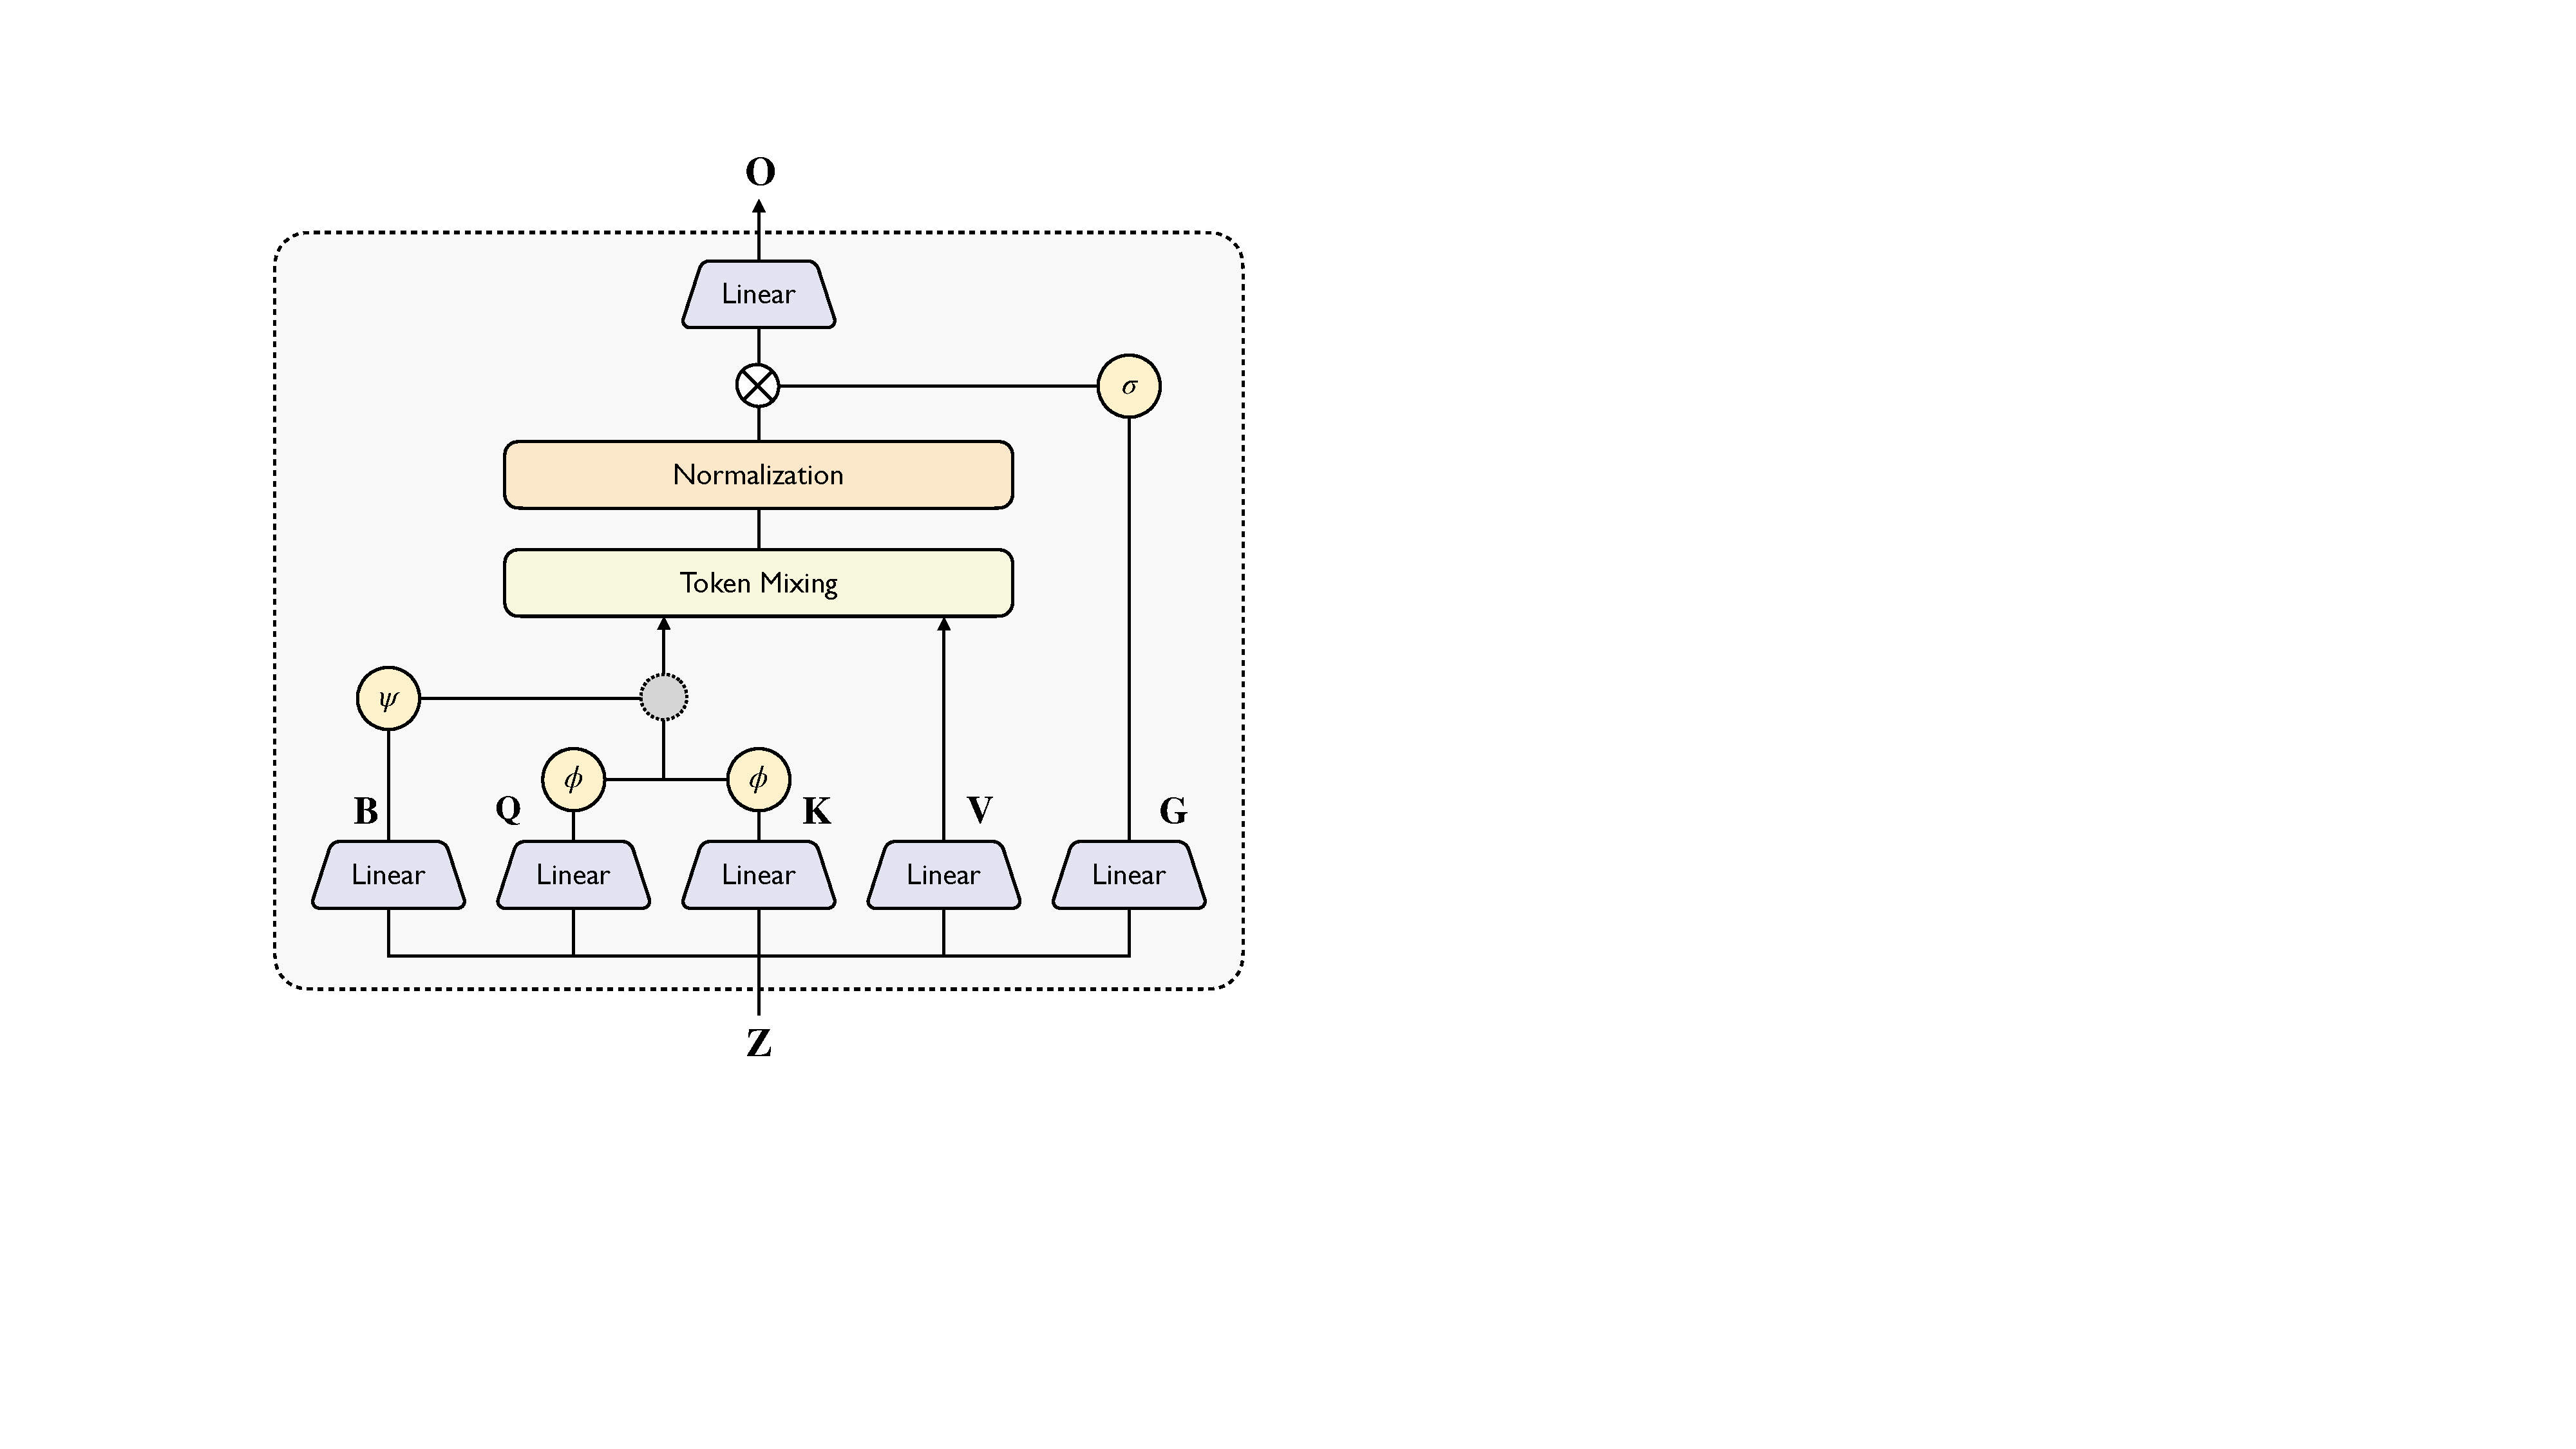
\includegraphics[width=0.5\linewidth]{figures/linear_attention.pdf}
%     \caption{The \texttt{LinearTriangularAttention} module.}
%     \label{fig:linear_attention}
% \end{figure}


% \begin{figure}[h]
%     \centering
%     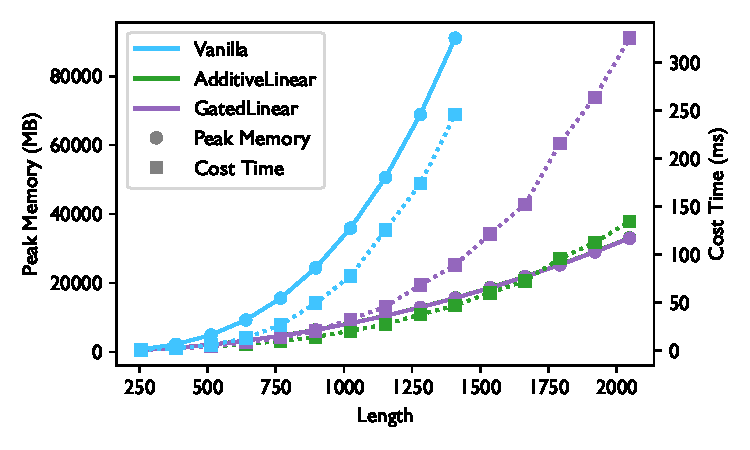
\includegraphics[width=0.5\linewidth]{figures/bench_kernel.pdf}
%     \caption{The benchmark of different attention modules.}
%     \label{fig:bench_kernel}
% \end{figure}






\subsection{Large Scale Data Distillation}
\label{sec:data_scaling}

In this section, we describe the data curation process for \texttt{SeedFold}. Detailed statistics are provided in Table~\ref{tab:data_stats}. We conducted large-scale data distillation to expand the training dataset to $26.5$M, which is $147$ times the size of the experimental dataset ($0.18$M). The motivation behind large-scale distillation stems from the paradigm shift from AlphaFold2 to AlphaFold3, where the inductive bias within the structure module is eliminated. AlphaFold2 employs the Invariant Permutation Attention (IPA) module to conduct reasoning in Euclidean space. In AlphaFold3, this module has been replaced with a general-purpose Transformer. Nevertheless, Transformers require large amounts of data and fail to generalize well when the dataset is small~\cite{dosovitskiy2020image}.

% \todoq{the captions of tables and figures need to be detailed enough so that they're self-contained}
\begin{table}[t]
    \centering
    \caption{Dataset Statistics. The training set can be divided into two parts: the experimental dataset and the distillation dataset. We sample from these two types of datasets with equal probability.}
    \label{tab:data_stats}
    \begin{tabular}{cccc}
        \toprule
        \textbf{Dataset} & \textbf{Type} & \textbf{\#Samples} & \textbf{Weight} \\
        \midrule
        PDB & Experimental & $180,540$ & $0.50$ \\
        AFDB & Distillation & $3,326,991$ & $0.08$ \\
        % Mgnify(v1) & Distillation & $23,075,211$ & $0.08$ \\
        % Mgnify(v2) & Distillation & $18,454,980$ & $0.34$ \\
        Mgnify & Distillation & $23,075,211$ & $0.42$ \\
        \bottomrule
    \end{tabular}
\end{table}


The training set we used can be divided into three parts: 
\begin{itemize}
    \item \textbf{Protein Structures} We utilized Boltz's data processing pipelines~\cite{passaro2025boltz}, with PDB structures~\cite{berman2000protein} included up to the training date cutoff of 2021-09-30. Each chain and interface is assigned to a cluster. During training, samples are weighted by both molecular type and cluster size to ensure balanced representation.
    \item \textbf{AFDB Dataset} We obtained $3.3$M structures from the AFDB database, an opensource dataset which is generated by AlphaFold2~\cite{varadi2022alphafold}. We first performed chain sequence clustering with a minimum sequence identity of $0.5$, and then filtered out structures with a pLDDT score below $0.8$. We employed the AFDB dataset as the source for short monomers. Specifically, we first determine whether to sample monomers shorter than $200$ with a probability of $0.08$, and then perform uniform sampling of a chain within the specified length range.
    \item \textbf{Mgnify Dataset} We constructed a large-scale distillation dataset based on the Mgnify dataset~\cite{mitchell2020mgnify,evans2021protein}. We first filtered out sequences with fewer than $200$ residues. The sequences were clustered using MMSeqs~\cite{steinegger2017mmseqs2} with a minimum sequence identity of $0.3$. We employed \texttt{colabfold\_search}~\cite{mirdita2022colabfold} to generate multiple sequence alignments (MSAs) from the \texttt{uniref30\_db} and \texttt{colabfold\_envdb} sequence databases. We used OpenFold~\cite{ahdritz2024openfold} to infer high-quality protein structures using AlphaFold2's official weights. % The AlphaFold2 team has released 5 models, among which \texttt{model\_1} and \texttt{model\_2} require templates. We ran all 5 models to avoid bias introduced by any specific model.
\end{itemize}




Here we briefly discuss the differences between the AFDB dataset and the MGnify dataset from three perspectives: the source, the diversity, and the length. (i) AFDB comprises AlphaFold-predicted 3D structures of proteins derived from UniProt sequences~\cite{uniprot2019uniprot}, whereas MGnify is a metagenomic dataset containing microbiome data from environmental microbial populations~\cite{mitchell2020mgnify}. (ii) From the perspective of model training, sample diversity is of greater concern. Our examination of the MGnify dataset revealed that among its $23$ million samples, only $2$ million could be assigned to clusters in the AFDB, thereby highlighting the sequence diversity. (iii) Figure~\ref{fig:data_length_dist} (in Appendix \ref{appendix:data}) presents the length distribution of the two distillation datasets, with the AFDB dataset having a median length of $95$ and the MGnify dataset a median length of $435$. This difference indicates that the Mgnify dataset may be beneficial for modeling long proteins.



